\documentclass[a4paper]{report}
\usepackage[utf8]{inputenc}
\usepackage{graphicx}
\usepackage{pdfpages}
\usepackage{lmodern}
\usepackage{txfonts} %Times New Roman
\usepackage[T1]{fontenc}
\usepackage{hyperref}


 
\title{Rusty Steam}
\author{Martin Strapko \\ Peter Šulík}
\date{\today}
\begin{document}
\maketitle

\tableofcontents
 
% \section*{Game In Short - with pictures}

% Zoom becouse you can.
% \begin{center}
% 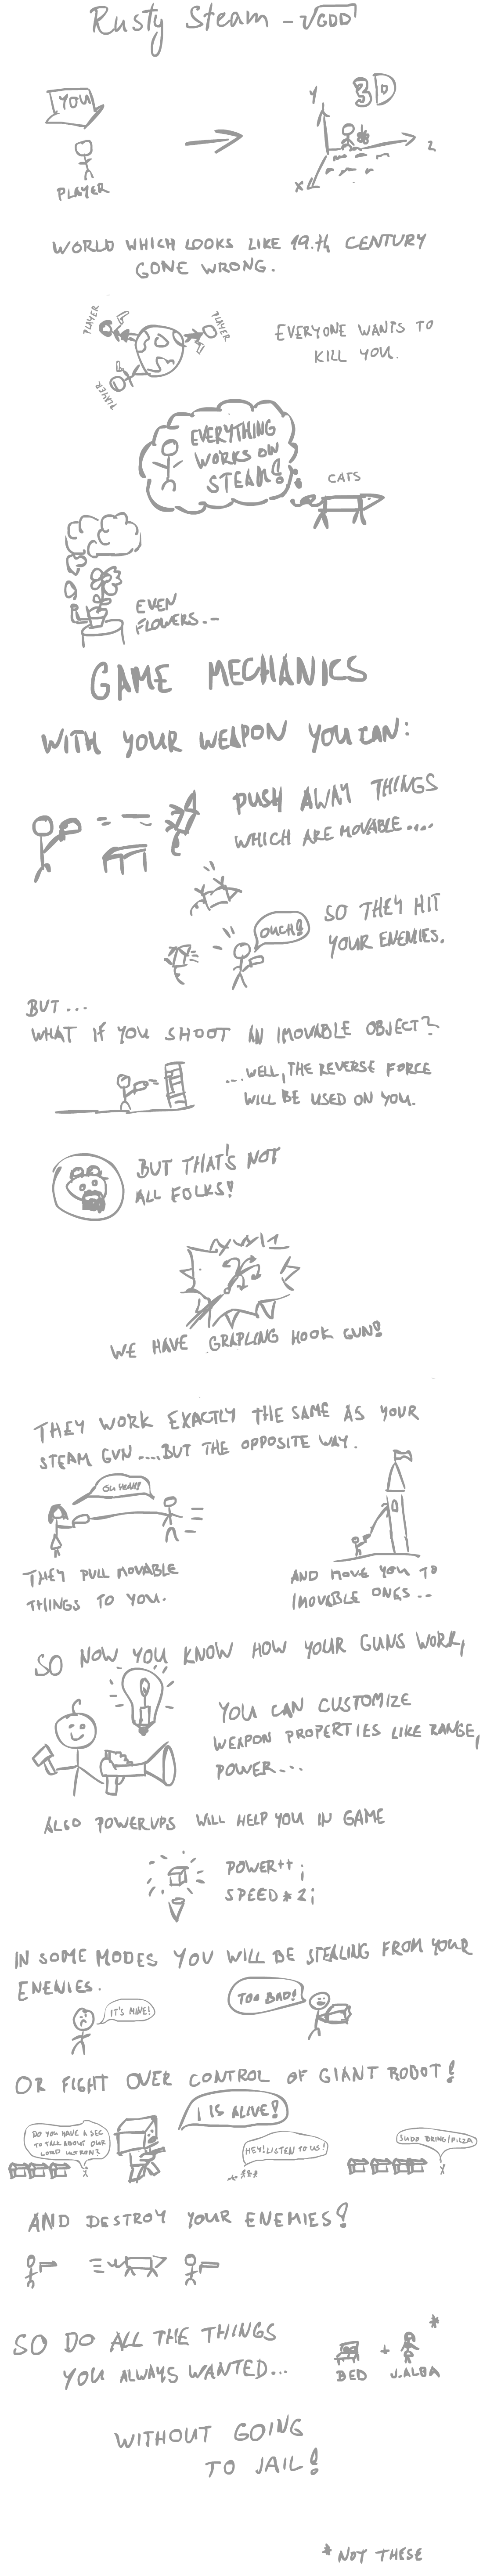
\includegraphics[width=\textwidth,height=\textheight,keepaspectratio]{about}
% \end{center}


% dfsgf


% \vspace*{-15cm}
% 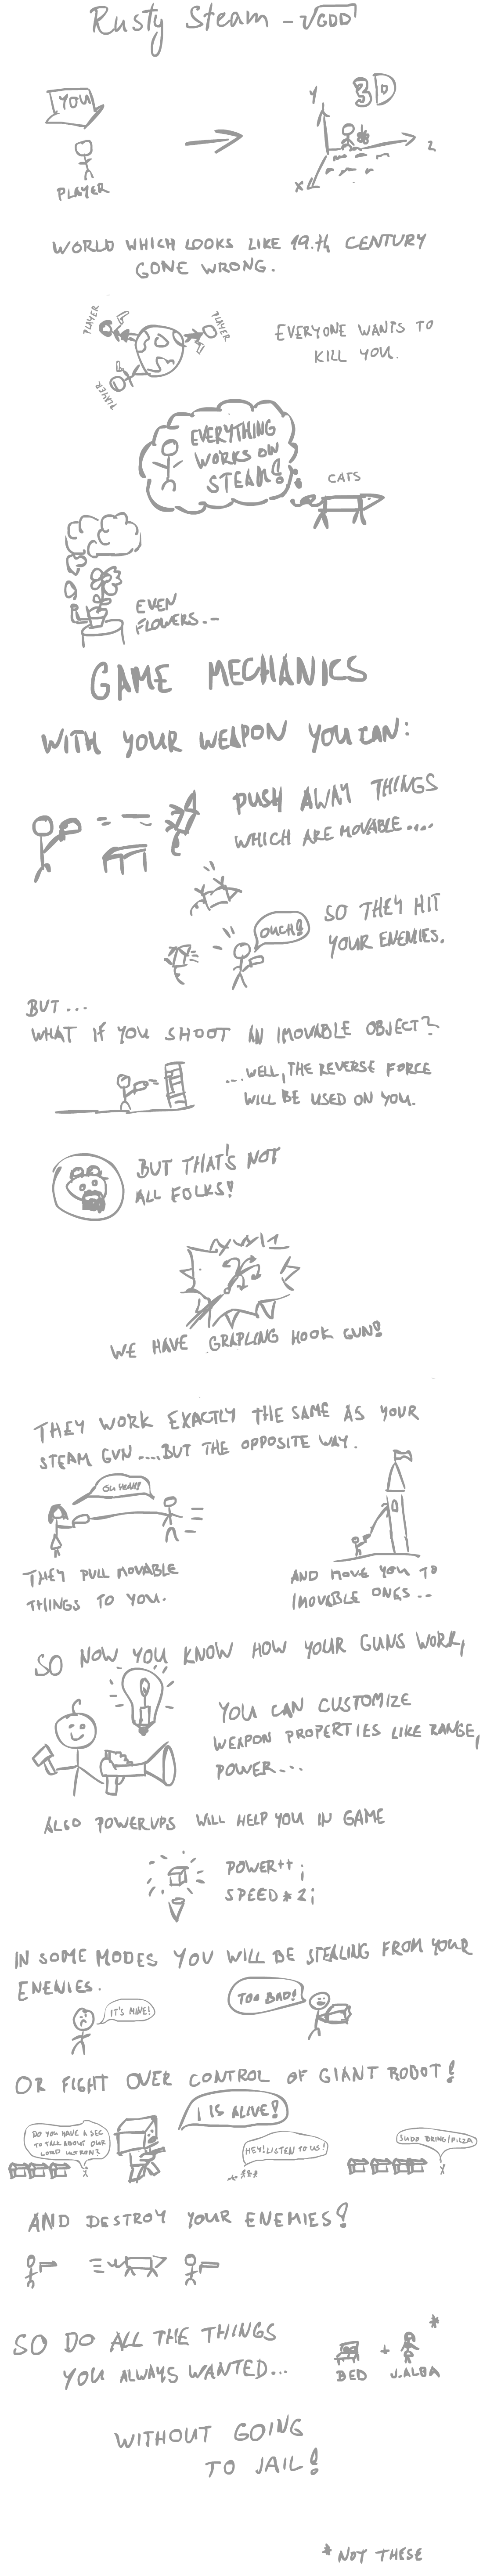
\includegraphics[width=\textwidth,keepaspectratio]{about}
% \vspace*{-\paperheight}
% 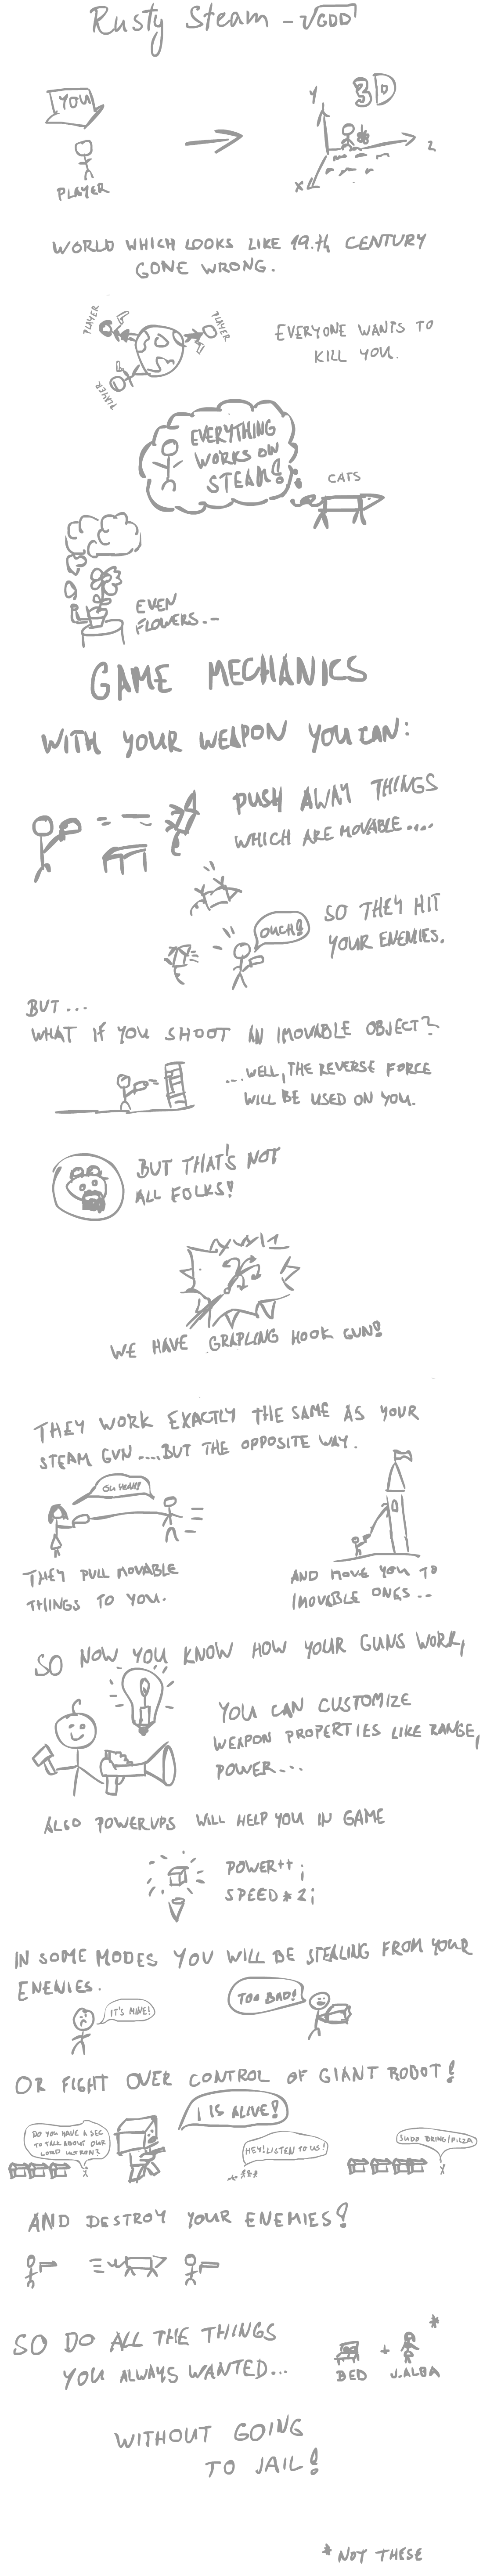
\includegraphics[width=\textwidth,keepaspectratio]{about}
% \vspace*{-\paperheight minus \paperheight}
% 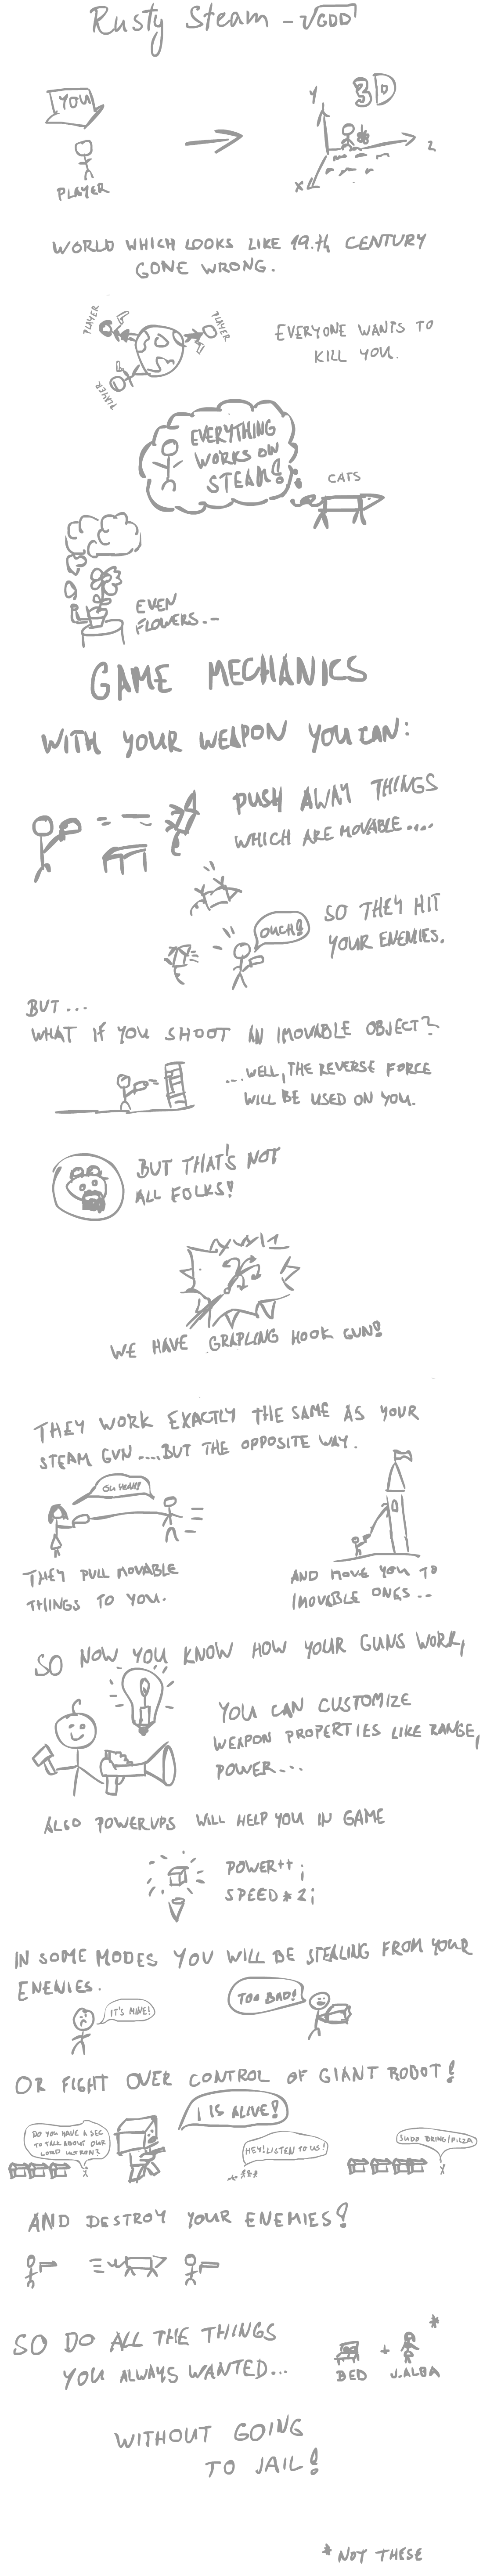
\includegraphics[width=\textwidth,keepaspectratio]{about}

\begin{center}
  \makebox[\textwidth]{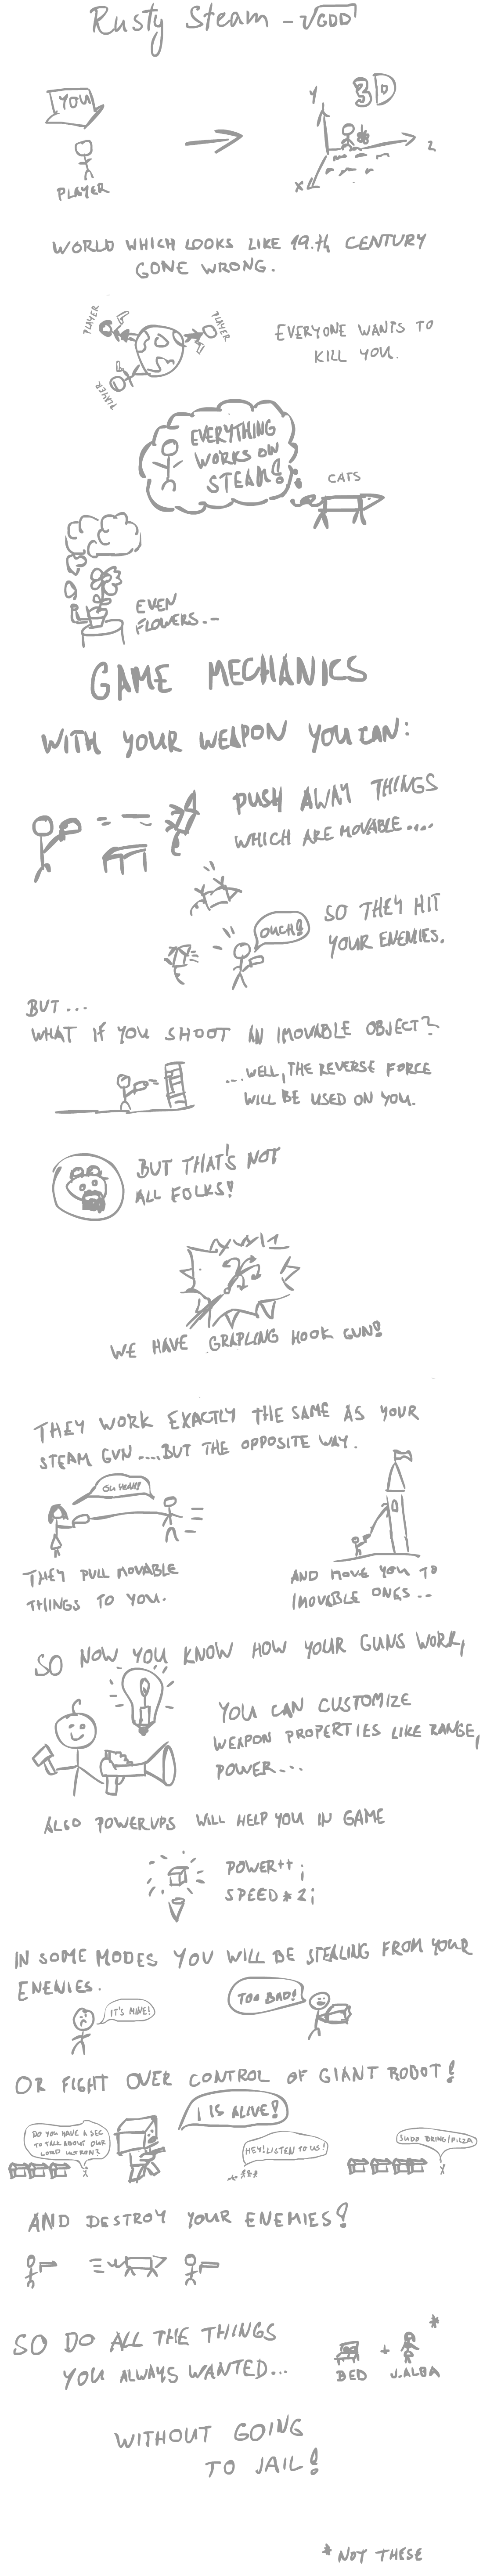
\includegraphics[width=\paperwidth]{about}}
\end{center}

\begin{center}
\vspace*{-\paperheight}
  \makebox[\textwidth]{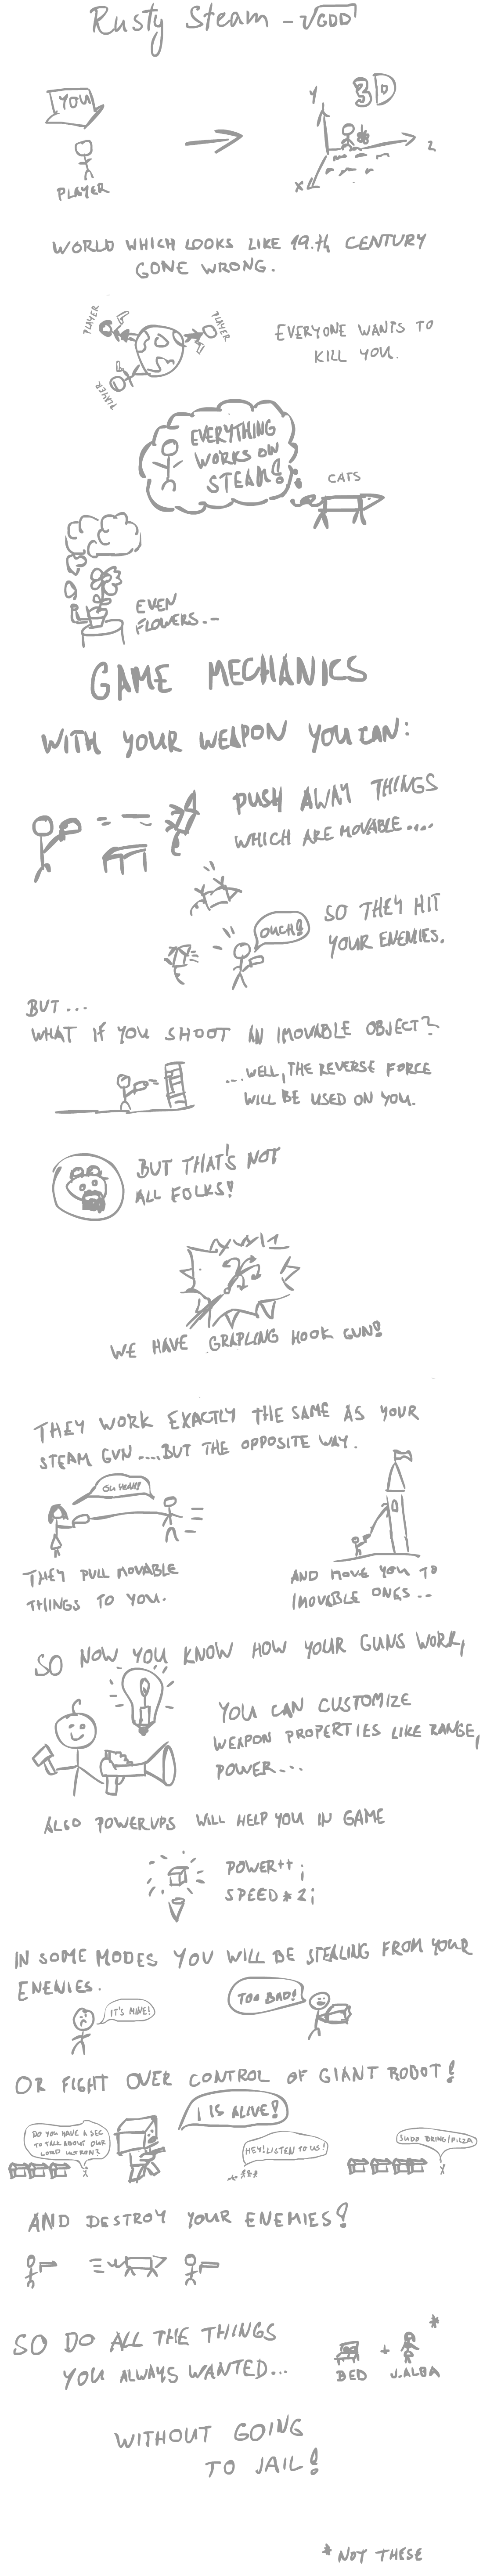
\includegraphics[width=\paperwidth]{about}}
\end{center}

\begin{center}
\vspace*{-\paperheight}\vspace*{-\paperheight}
  \makebox[\textwidth]{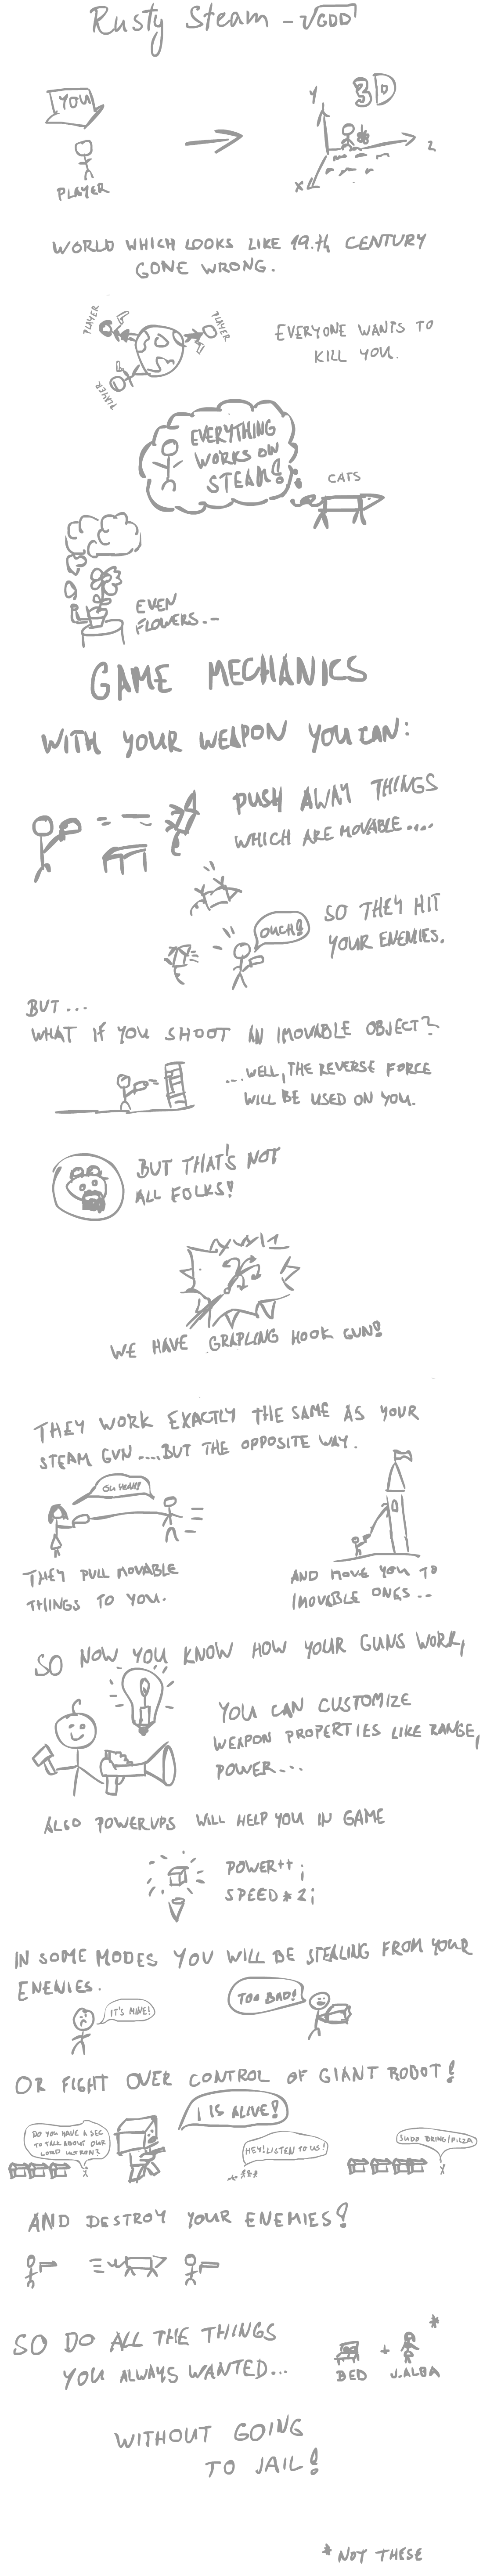
\includegraphics[width=\paperwidth]{about}}
\end{center}

\begin{center}
\vspace*{- \paperheight}\vspace*{-\paperheight}\vspace*{-\paperheight}
  \makebox[\textwidth]{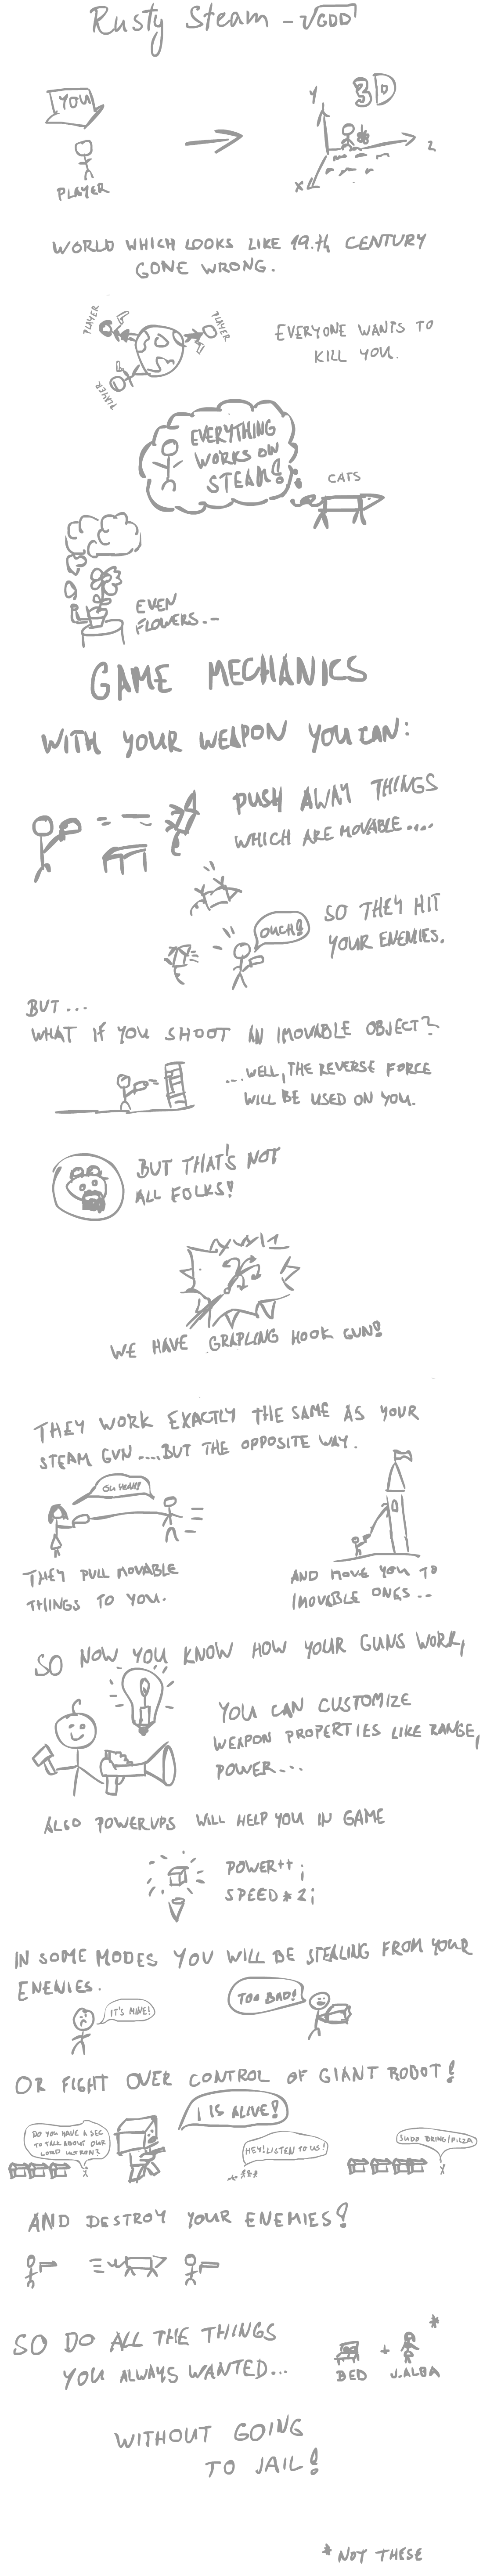
\includegraphics[width=\paperwidth]{about}}
\end{center}




\chapter{Story}
Prostredie, v ktorom sa hra odohráva je neznáma krajina 21. storočia, kde sa vybralo ľudstvo inou historickou cestou ako cestou elektriny a ostalo verné energii pary. Tú využívaju takmer všetky pristroje. Je to  prostredie v ktorom, je každý druhý občan tejto krajiny kutil, ktorý experimentuje a vytvára si rôzne šikovné prístroje. To sa však nepáči vláde, ktorá chce mať pod kontrolou tvorbu týchto prístrojov a aj predaj. Vznikajú agresivné potičky, ktoré sú na dennom poriadku, v ktorých si rôzne kutilské klany tovarní dokazujú, kto vyrába lepšie prístroje. V jednej z nich sa ocitá aj hráč. 

\section{Structure}
Hra je určená pre hru viacerých hráčov, ktorý bojujú v určitej \"aréne\" alebo na ohraničenom území. Hráči neobjavujú nové časti deju - skôr sú len vhodený do prostredia, ktorého história a pribéhy postáv v ňom bojujúcich sú povedané v popiskoch/cutscénach pri výbere postáv, či levelov. Pre jednotlivé Game Mody a pre jednotlivé postavy bude vytvorený príbeh vyscetlujúci ich pozadie.

\section{Capture The Flow}
Tento konflikt vznikol kvôli vedeckej komunite, ktorá sa v určitom období rozdelila na dva smery. Jeden, za ktorým stál známy vedec Ed Tyson, hlásajúci jednosmerný prúd pary. Na druhej strane stála vedkyňa La Tess, ktorá tvrdila, že budúcnosť patrí striedavému prúdu pary. Obaja vedci vyrobili určité množstvo jedného aj druhého typu pary, tie však ukradli nadšenci jednotlivých smerov. Tak ako to aj z našej histórie poznáme sa po dlhodobých diskusiách oboch strán naskytlo riešenie - vojna. Alebo aspoň tak si to vysvetlili obyvatelia, ktorí chcú dokázať pravdu svojho presvedčenia tým, že ukradnú tej druhej skupine nádoby obsahujúce ich typ pary a prinesú do svojej zákládni, kde ich zničia. Keď jeden z týchto tímov príde o všetky zásoby pary - prehrá argument. A tak keďze hráč je členom jedného z týchto smerov tak ovplyvní buducnosť, ktorý typ pary je lepší. Tradične logckými argumentami.

\section{King of the Kong}
Pri jednom z konfiktov sa splnili predpovede mnohých konšpirátorov. Vláda naozaj začala stavať stroj, pomocou ktorého chcela ukludniť nepokoje a nastoliť poriadok. Volala sa KONG.(Kolosálna ozaj nie gorila/kontrolovany obor na gaunerov) Bol to obrovitánsky robot, ktorý pripomínal žirafu. To čo však vláda netušila, bolo, že jej tajnú zbráň obyvatelia našli a chceli sa jej zmocniť. Rozhadáli sa však dve strany mesta - každá zo strán ho chcela mať na svojej strane kde by slúžila ako vyhliadková veža. Kompromis v strede zrejme nebol dobrý nikomu a tak sa hráč stáva súčasťou boja, kde dve súperiace strany bojoujú o nadvladu nad KONGom. 
// Lol. poznámka pomimo: existuje kapela \href{https://youtu.be/dDRHx4cPgbE?t=50s}{Steam Powered Giraffe} . 
 

\chapter{Feature Listing}
\begin{itemize}
  \item 3D First Person Shooter
  \item Grappling Hooks
  \item Enviroment Control
  \item Multiplayer
  \item Weapon Customization
  \item Different Characters
  \item Tutorial
\end{itemize}

\chapter{Requirements}
\begin{itemize}
  \item Internet Connection - Hra je primárne určená na hranie s ostatnými hráčmi. Pri tvorbe hernej session využíva Unity masterserver pre vytváranie a nájdenie hier.
  \item Windows/Linux/OSX
\end{itemize}


\chapter{Gameplay}
\section{Game Mechanics}
 Hlavnou mechanikou hry je priťahovanie a odtláčanie. Hráči budú schopný pomocou zbraní pohybovať rôzne časti prostredia, toto zahŕňa napríklad aj ostatných hráčov. Pri použití voči statickým prvkom prostredia je automaticky použitá opačná sila na hráča - teda napríklad hráč, ktorý chcel odhodiť nepohyblivú stenu sa odhodí od nej. Hráči sa môžu klasicky pohybovať po prostredí a majú určitú formu ukazatela životov. Hráčom znižuje množstvo životov sila, ktorá na nich pôsobí pri kolízií s objektami - či už statickými (stena, zem) alebo pohyblivými (rôzne objekty). Taktiiež je možno nepriateľom ubrať životy pomocou ďalších možných spôsobov napríklad polohovaním nepriateľa do určitých zón alebo pomocou ripshotu - viď nižšie.  Hra má pomerne vysoké tempo, preto je vhodná hlavne pre skúsených hráčov FPS hier. Použitie odpudivej sily je vrámci dostrelu okamžité, narozdiel od priťažlivej, ktorá sa pohybuje určitou rýchlosťou do určitej vzdialenosti dostrelu.

\section{Game Mode}
Hodnotenie hráčov záleži od zvoleného herného módu, aj keď zabíjanie hráčov je dôležité v oboch módoch, jeho dopad sa líši. Hráči sa budú rozlišovať farbou modelu podľa tímu do ktorého patria.
\subsection{Team Deathmatch}
Hráči musia nazbierať stanovený počet fragov skôr ako nepriateľský tím. Tie získajú zabitím nepriateľov pomocou prostredia, vyhodenia z mapy alebo spoluprácou so svojími spoluhráčmi na nejakom combe.

\subsection{Capture The Flow}
Klasický mód Capture The Flag.
Skóre tímov sa počíta v množstve vlajok/špeciálnych objektov, ktoré odniesli z nepriateľskej základne do svojej. Vlajka z človeka spadne ak bude trafení nejakým objektom (toto trafenie nemusí byť smrteľné) alebo zabití.

\subsection{King of the Kong}
Hra má podobný priebeh ako Team Deathmatch len v určitých intervaloch sa spawne neutrálna jednotka, Kong, ktorá periodický pridáva body tímu, ktorý ho ovláda. Ovládnutie Konga je zložitý proces pri ktorom budú hráči musieť spolupracovať tak aby sa dostali na určitú pozíciu, na ktorej je Kong ovládany. Úlohou druhého tímu je prebrať Konga na svoju stranu zneškodnením hráča, ktorý Konga ovláda a dosadení svojho vlastného spoluhráča, ktorý ho bude ovládať. 

\section{Controls}
Hra sa primárne ovláda pomocou klávesnice a myši. Všetky akcie hráča sú meniteľné na základe preferencií hráča. 

\section{Combos}
Mechaniky hry umožnia hráčom v multiplayeri pomocou fyziky robiť kombá, ako napríklad vystreliť hráča ako projektil alebo takzvaný ripshot, roztrhnutie hráča keď ho naraz pritiahujú dvaja rôzny hráči. Podhadzovanie objektov druhému hráčovi ako dočasné plošiny od ktorých môže odskočiť. 

\section{Drops to Powerups}
Vo svete sa budú spawnovať powerupy, ktoré dočasne vylepšia atribúty hráča alebo jeho zbraní. Rýchlejšie projektily, pohyb, zdravie, neviditeľnosť, imunita a tak podobne.

\section{Weapon Customization}
Z menu budú mať hráči možnosť poupravovať si zbrane podľa vlastného štýlu hrania a chute. Budú mať maximálny počet bodov, ktoré budú mocť rozdeliť medzi rôzne parametre zbrane ako dostrel, rýchlosť projektilu, šírka projektilu a ďalšie.
 
\chapter{Visual}
\section{Art Style}
Hlavnou grafickou témou hry bude steampunk, a všetky prvky hry budú ladené podľa tejto témy. Farebna paleta by mala byt pastelová, taktiež by modely mali byť relativne jednoduché a zložene z málo polygónov a detaily objektov by mali byť v textúrach. Primarny smer designu postáv i objektov by mal byť ladený do cartoon/chibi štýlu, kde sa upúšta od realizmu a váha je skôr na disproporcii(velké hlavy, ruky, nohy), ktorá nahráva cute štýlu, takmer ako pre deti. Avšak určite pri RIPshotoch a iných typoch smrti by bol vyborné odskušať kontrast s naturalizmom - nešetriť krvou a chrbticami bez hláv. 

\section{Character Selection}
 Hráči si môžu vybrať výzor svojej postavy pred začaťím hry z predvyrobených postáv. Primárne by výzor postavy nemal ovplyvňovať gameplay. 

\section{User Interface}
\subsection{Menus}
\begin{itemize}
  \item Vytvorenie hernej session
  \item Vyhľadanie aktívnych herných session
  \item Herné lobby
  \item Nastavenie rozlíšenia
  \item Nastavenie ovládania
  \item Výber postavy
  \item Výber a customizácia zbraní
  \item Volba mena
\end{itemize}
 
\subsection{Gameplay}
Počas hry budú mať hráči prístup k rôznym indikátorom: vidiet indikátory zobrazujúce pripravenosť zbraní, skóre oboch tímov a 3D radar na ktorom sa im bude zobrazovať poloha spojencov a nepriateľov.
\begin{itemize}
  \item Ukazovateľ životov
  \item Pripravenosť zbraní
  \item 3D Minimapa
  \item Chat
  \item Mená hráčov
\end{itemize} 


\end{document}
